\documentclass[11pt]{amsart}



\usepackage{mathrsfs}
\usepackage{amsmath, amscd, amsthm,amssymb, thmtools, amsfonts, verbatim,subfigure}
\usepackage[mathcal]{eucal}
\usepackage{hyperref}
\usepackage[cmtip, arrow, all]{xy}
\usepackage{pb-diagram ,pb-xy}
\usepackage{graphicx}
\usepackage{epstopdf}
%\DeclareGraphicsRule{.tif}{png}{.png}{`convert #1 `basename #1 .tif`.png}

%Use Palatino and Euler fonts
\usepackage{mathpple}



\textwidth=14.5cm  \oddsidemargin=1cm \evensidemargin=1cm
%\setlength{\parskip}{7pt}
\setlength{\headsep}{20pt}




\title[The McKean-Singer Formula via Equivariant Quantization]{McKean-Singer via Equivariant Quantization}
\author{Eugene Rabinovich}
\address{Department of Mathematics \\ University of California, Berkeley}
\email{erabin@math.berkeley.edu}

\date{}


\renewcommand{\Re}{\op{Re} } 

\newcommand{\eps}{\varepsilon}
\renewcommand{\epsilon}{\varepsilon}
\newcommand{\xto}{\xrightarrow}
\newcommand{\E}{\mscr{E}}
\newcommand{\what}{\widehat}
\newcommand{\til}{\widetilde}
\newcommand{\mscr}{\mathscr}
\newcommand{\br}{\overline}
\newcommand{\iso}{\cong}
\newcommand{\C}{\mathbb C}
\newcommand{\N}{\mathbb N}
\newcommand{\Q}{\mbb Q}
\newcommand{\rarr}{\rightarrow}
\newcommand{\larr}{\leftarrow}
\newcommand{\norm}[1]{\left\| #1 \right\|}
\newcommand{\Oo}{\mscr O}
\newcommand{\Z}{\mathbb Z}
\newcommand{\defeq}{\overset{\text{def}}{=}}
\newcommand{\into}{\hookrightarrow}
\newcommand{\op}{\operatorname}
\newcommand{\mbf}{\mathbf}
\newcommand{\mbb}{\mathbb}
\newcommand{\mf}{\mathfrak}
\newcommand{\mc}{\mathcal}
\newcommand{\from}{\leftarrow}
\newcommand{\ip}[1]{\left\langle #1 \right\rangle}
\newcommand{\abs}[1]{\left| #1 \right|}
\newcommand{\cmod}{\overline {\mc M}}
\newcommand{\R}{\mbb R}
\renewcommand{\d}{\mathrm{d}}

\newcommand{\liminv}{ \varprojlim }
\newcommand{\limdir}{\varinjlim}
\newcommand{\dirlim}{\varinjlim}
\renewcommand{\Bar}{\op{Bar}}
\newcommand{\dbar}{\br{\partial}}
\renewcommand{\Im}{\op{Im}}
\newcommand{\RHom}{\mbb R\Hom}
\newcommand{\REnd}{\mbb R \End}



\DeclareMathOperator{\dens}{Densities}
\DeclareMathOperator{\Aut}{Aut} \DeclareMathOperator{\End}{End}
\DeclareMathOperator{\Supp}{Supp} 
\DeclareMathOperator{\Sym}{Sym} \DeclareMathOperator{\Hom}{Hom}
\DeclareMathOperator{\Spec}{Spec} \DeclareMathOperator{\Deg}{Deg}
\DeclareMathOperator{\Diff}{Diff}   \DeclareMathOperator{\Ber}{Ber}
\DeclareMathOperator{\Tr}{Tr} \DeclareMathOperator{\Cyc}{Cyc}
\DeclareMathOperator{\Or}{Or}\DeclareMathOperator{\Ker}{Ker}
\DeclareMathOperator{\Mat}{Mat} \DeclareMathOperator{\Ob}{Ob}

\def\cA{\mathcal A}\def\cB{\mathcal B}\def\cC{\mathcal C}\def\cD{\mathcal D}
\def\cE{\mathcal E}\def\cF{\mathcal F}\def\cG{\mathcal G}\def\cH{\mathcal H}
\def\cI{\mathcal I}\def\cJ{\mathcal J}\def\cK{\mathcal K}\def\cL{\mathcal L}
\def\cM{\mathcal M}\def\cN{\mathcal N}\def\cO{\mathcal O}\def\cP{\mathcal P}
\def\cQ{\mathcal Q}\def\cR{\mathcal R}\def\cS{\mathcal S}\def\cT{\mathcal T}
\def\cU{\mathcal U}\def\cV{\mathcal V}\def\cW{\mathcal W}\def\cX{\mathcal X}
\def\cY{\mathcal Y}\def\cZ{\mathcal Z}

\def\AA{\mathbb A}\def\BB{\mathbb B}\def\CC{\mathbb C}\def\DD{\mathbb D}
\def\EE{\mathbb E}\def\FF{\mathbb F}\def\GG{\mathbb G}\def\HH{\mathbb H}
\def\II{\mathbb I}\def\JJ{\mathbb J}\def\KK{\mathbb K}\def\LL{\mathbb L}
\def\MM{\mathbb M}\def\NN{\mathbb N}\def\OO{\mathbb O}\def\PP{\mathbb P}
\def\QQ{\mathbb Q}\def\RR{\mathbb R}\def\SS{\mathbb S}\def\TT{\mathbb T}
\def\UU{\mathbb U}\def\VV{\mathbb V}\def\WW{\mathbb W}\def\XX{\mathbb X}
\def\YY{\mathbb Y}\def\ZZ{\mathbb Z}

\def\sA{\mathscr A}\def\sB{\mathscr B}\def\sC{\mathscr C}\def\sD{\mathscr D}
\def\sE{\mathscr E}\def\sF{\mathscr F}\def\sG{\mathscr G}\def\sH{\mathscr H}
\def\sI{\mathscr I}\def\sJ{\mathscr J}\def\sK{\mathscr K}\def\sL{\mathscr L}
\def\sM{\mathscr M}\def\sN{\mathscr N}\def\sO{\mathscr O}\def\sP{\mathscr P}
\def\sQ{\mathscr Q}\def\sR{\mathscr R}\def\sS{\mathscr S}\def\sT{\mathscr T}
\def\sU{\mathscr U}\def\sV{\mathscr V}\def\sW{\mathscr W}\def\sX{\mathscr X}
\def\sY{\mathscr Y}\def\sZ{\mathscr Z}

\def\bA{\mathbf A}\def\bB{\mathbf B}\def\bC{\mathbf C}\def\bD{\mathbf D}
\def\bE{\mathbf E}\def\bF{\mathbf F}\def\bG{\mathbf G}\def\bH{\mathbf H}
\def\bI{\mathbf I}\def\bJ{\mathbf J}\def\bK{\mathbf K}\def\bL{\mathbf L}
\def\bM{\mathbf M}\def\bN{\mathbf N}\def\bO{\mathbf O}\def\bP{\mathbf P}
\def\bQ{\mathbf Q}\def\bR{\mathbf R}\def\bS{\mathbf S}\def\bT{\mathbf T}
\def\bU{\mathbf U}\def\bV{\mathbf V}\def\bW{\mathbf W}\def\bX{\mathbf X}
\def\bY{\mathbf Y}\def\bZ{\mathbf Z}

\def\fA{\mathfrak A}\def\fB{\mathfrak B}\def\fC{\mathfrak C}\def\fD{\mathfrak D}
\def\fJ(E){\mathfrak E}\def\fF{\mathfrak F}\def\fG{\mathfrak G}\def\fH{\mathfrak H}
\def\fI{\mathfrak I}\def\fJ{\mathfrak J}\def\fK{\mathfrak K}\def\fL{\mathfrak L}
\def\fM{\mathfrak M}\def\fN{\mathfrak N}\def\fO{\mathfrak O}\def\fP{\mathfrak P}
\def\fQ{\mathfrak Q}\def\fR{\mathfrak R}\def\fS{\mathfrak S}\def\fT{\mathfrak T}
\def\fU{\mathfrak U}\def\fV{\mathfrak V}\def\fW{\mathfrak W}\def\fX{\mathfrak X}
\def\fY{\mathfrak Y}\def\fZ{\mathfrak Z}\def\fg{\mathfrak g}\def\fh{\mathfrak h}

\declaretheoremstyle[
spaceabove=7pt, spacebelow=7pt,
headfont=\normalfont\bfseries,
notefont=\mdseries, notebraces={(}{)},
bodyfont=\itshape,
postheadspace=5pt,
headpunct = .
]{thm}

\declaretheoremstyle[
spaceabove=7pt, spacebelow=7pt,
headfont=\normalfont\bfseries,
notefont=\mdseries, notebraces={(}{)},
bodyfont=\itshape,
postheadspace=10pt,
headpunct = .
]{def}

\declaretheoremstyle[
spaceabove=4pt, spacebelow=7pt,
headfont=\itshape,
postheadspace=5pt,
headpunct = :,
postheadspace = 3pt, qed = $\lozenge$
]{rem}

\declaretheorem[numbered = no, style = thm]{claim}
\declaretheorem[numbered = no, style = thm, name = Theorem]{utheorem}
\declaretheorem[numbered = no, style = thm, name = Main Theorem]{thmmain}
\declaretheorem[numbered = no, style = thm, name = Proposition]{uproposition}
\declaretheorem[numbered = yes, parent = section, style = thm]{theorem}
\declaretheorem[numbered = no, style = thm, name = Theorem A]{thmA}
\declaretheorem[numbered = no, style = thm, name = Theorem B]{thmB}
\declaretheorem[numbered = no, style = thm, name = Theorem C]{thmC}
\declaretheorem[numbered = no, style = thm, name = Theorem D]{thmD}
\declaretheorem[numbered = no, style = thm]{conjecture}
\declaretheorem[numbered = no, style = thm, name = Corollary]{ucorollary}
\declaretheorem[numbered = no, style = thm, name = Lemma]{ulemma}

\declaretheorem[sibling = theorem, style = thm, name = Theorem/Definition]{thm-def}
\declaretheorem[sibling = theorem, style = thm]{proposition}
\declaretheorem[sibling = theorem, style = thm]{lemma}
\declaretheorem[sibling = theorem, style = thm]{notation}
\declaretheorem[sibling = theorem, style = thm, name = Definition-Lemma]{deflem}
\numberwithin{equation}{section}


\declaretheorem[sibling = theorem, style = def]{definition}
\declaretheorem[numbered = no, style = def, name = Definition]{udefinition}


\declaretheorem[numbered = no, style = rem]{remark}
\declaretheorem[numbered = no, style = rem]{remarks}
\declaretheorem[numbered = no, style = rem]{example}

%%This document
\newcommand{\cinfty}{C^{\infty}}
\newcommand{\GF}{Q^{GF}}


\newcommand\ind{\operatorname{ind}}
\newcommand\Str{\operatorname{Str}}
\newcommand\coker{\operatorname{coker}}
\newcommand\Mor{\operatorname{Mor}}
\newcommand\Obcl{\operatorname{Obs}^{cl}(U)}
\newcommand\Obq{\operatorname{Obs}^{q}(U)}
\renewcommand{\L}{\mathscr{L}}
\begin{document}
\maketitle
\section{Introduction}
The aim of this note is to present a proof, using the language of factorization algebras, and in particular the index theorem in Chapter 7 of \cite{ref: othesis}, of the following 
\begin{theorem}[McKean-Singer]
	Let $V$ be a Hermitian, $\Z_2$-graded vector bundle on a closed Riemannian manifold $M$, with $|dx|$ the Riemannian volume form on $M$. Let $D$ be a self-adjoint Dirac operator on $V$, with $k_t$ the heat kernel of $D^2$. Then
	\begin{equation}
		\label{eq: mcs}
		\ind(D)=\int_M \Str(k_t(x,x)) |dx|.
	\end{equation}
\end{theorem}

The actual McKean-Singer theorem works for non-self-adjoint Dirac operators as well, but our proof will require $D$ to be self-adjoint. We will give definitions of all of the objects in the theorem shortly, but first a bit of philosophy. This theorem gives us a relationship between a global, analytic quantity (the index of a Dirac operator) and a local, physical quantity (the super-trace of a heat kernel). This is what the index theorem is most famous for. We will see that the theorem of Gwilliam is similar in nature: it describes two ways to compute the obstruction to quantizing a field theory equivariantly with respect to the action of an $L_\infty$ algebra. One involves Feynman diagrams (which involve heat kernels), and the other is a global characterization (which will give us the index). This is, very roughly speaking, why we are able to use the theorem relating to field theory to prove an index-type theorem.


\section{Generalized Laplacians, Heat Kernels, and Dirac Operators}
We present here a list of definitions and results relevant to the result. Throughout, $M$ is a Riemannian manifold with Riemannian volume form $|dx|$. We let $V\to M$ be a vector bundle, which we will eventually specialize to be $\Z_2$-graded. We let $\mathscr V$ be the sheaf of smooth sections of $V$. We always use normally-fonted letters for vector bundles and scripty letters for the sheaves of sections of the corresponding vector bundles.
\begin{definition}
	A \textbf{generalized Laplacian} is a differential operator
	\[
	H:\mathscr V(M) \to \mathscr V(M)
	\]
	such that 
	\[
	[[H,f],f] = -2|df|^2,
	\]
	where we are thinking of $C^\infty$ functions as operators given multiplication by those functions.
\end{definition}
Now we let $V$ be $\Z_2$-graded, and we denote by $V^{\pm}$ the plus or minus graded components of $V$.
\begin{definition}
	A \textbf{Dirac operator} on $V$ is a grading-reversing operator
	\[
	D: \mathscr V^\pm \to \mathscr V^\mp
	\]
	such that $D^2$ is a generalized Laplacian. If $V$ is a Hermitian bundle with inner product $(,)$, then we say that $D$ is \textbf{self-adjoint} if for all $s,r\in \mathscr V$, 
	\[
	\int_M (s,Dr)|dx| = \int_M(Ds,r)|dx|
	\]
\end{definition}
\begin{theorem}[The Heat Kernel]
	Let $V$ be a $\Z_2$-graded vector bundle with Dirac operator $D$. Write $H:=D^2$ for the generalized Laplacian corresponding to $D$. Then there is a unique \textbf{heat kernel} $k \in \Gamma(M\times M\times \R_{>0},V\boxtimes V^\vee)$ satisfying: 
	\begin{enumerate}
		\item 
		\[
		\frac{d}{dt}k_t + (H\otimes 1)k_t = 0
		\]
		\item For $s\in \Gamma(M, E)$,
		\[
		\lim_{t\to 0}\int_{y\in M} k_t(x,y) s(y) |dx| = s(x),
		\]
		where the limit is uniform over $M$ and is taken with respect to some norm on $V$.
	\end{enumerate}
	The heat kernel is the kernel of the operator $e^{-tH}$ in the sense that 
	\[
	\int_{y\in M} k_t(x,y)s(y) = (e^{-tH}s)(x).
	\]
\end{theorem}
\begin{definition}
	Let $D^+$ denote the restriction of a self-adjoint Dirac operator $D$ to the space of positively-graded sections, and similarly for $D^-$. Then, the \textbf{index} $\ind(D)$ of $D$ is $\dim(\ker(D^+))-\dim(\coker(D^+))$.
\end{definition}
The last definition we need to understand this theorem as stated is 
\begin{definition}
	If $\phi: V\to V$ is a grading-preserving endomorphism of the super-vector space $V$, then the \textbf{supertrace} $\Str(\phi)$ is defined to be 
	\[
	\Str(\phi) = \Tr(\phi\mid_{V^+})-\Tr(\phi\mid_{V^-})
	\]
\end{definition}
With these definitions in place, the statement of the McKean-Singer formula should be comprehensible. 
\section{Equivariant Quantization of Free Theories}
In this section, we assume familiarity with chapter 7 of \cite{ref: othesis}. All our notation will match that section, except that we will use $Q$ and $Q^{GF}$ to denote the differential and gauge-fixing operators of the full, cotangent theory. We will apply the general theory there to a specific example, which we now describe. In our context, since we are dealing with a Riemannian manifold, we will always use the Riemannian density to trivialize the bundle of densities.

\subsection{Motivation}
Our goal is to prove formula \ref{eq: mcs} using the techniques of chapter 7 of \cite{ref: othesis}, but it is worth commenting on the physical setup from which it arises. Given a Hermitian, $\Z_2$-graded vector bundle $V$ and  self-adjoint Dirac operator $D$ on $\mathscr V$, we can think of these data as specifying a free field theory with space of fields $\sV$ and action 
\[
S = \int \left( s, Ds\right)|dx|.
\] 
This action corresponds to the equation of motion $Ds=0$, which is obviously still satisfied if $s$ is replaced with $(1+\lambda )s$, where $\lambda\in \R$. Thus, the classical theory possesses a scaling symmetry, and we would like to see whether it persists at the quantum level. The obstruction to quantizing this symmetry is called the {\em scaling anomaly}. We expect to be able to find two ways of computing the scaling anomaly; comparing these two ways should give us formula \ref{eq: mcs}.

So, we have an action of the abelian Lie algebra $\R$ (which we may think of as an $L_\infty$-algebra, if we like) on $\sV$, given by $\lambda\cdot s = \lambda s$. As it stands, however, we do not have a setup which matches \cite{othesis}, where we need a {\em local} action of an {\em elliptic} $L_\infty$-algebra. The resolution of this conundrum is provided to us by Lemma 11.1.3.2 in \cite{ref: CG2}, which tells us that there is a homotopy equivalence between
\begin{enumerate}
\item the simplicial set of actions of an $L_\infty$-algebra $\mathfrak g$ on an elliptic $L_\infty$-algebra $\sM$, and
\item the simplicial set of local actions of $\mathfrak g \otimes \Omega^\bullet$ on $\sM$.
\end{enumerate}
Thus, we can choose any extension of the action of $\R$ on $\sV$ to an action of $\Omega^\bullet$ on $\sV$ and the choice will not matter homotopically. We therefore proceed to give one such extension next.

\subsection{The Main Example}
We continue to assume that $V$ and $D$ are as above. Based on the above discussion, we wish to find a local action of $\sL=\Omega^\bullet$ on $\E$, where $\E$ is the complex $\mathscr V^+ \overset{D^+}{\longrightarrow} \mathscr V^-$ with $\sV^+$ in degree 0, and we are thinking of $\Omega^\bullet$ and $\E$ as abelian dg Lie algebras.

To give an action of $\sL$ on $\E$, it will suffice to define a map
\[
[\cdot,\cdot]:\sL \otimes \E \to \E,
\]
with the elements of $\sL$ acting by differential operators and satisfying
\begin{enumerate}
\item The derivation property:
\[
Q([X,\phi]) = [dX, \phi] +(-1)^{\abs{X}}[X,Q\phi]
\]
\item The Jacobi identity:
\[
[X,[Y,\phi]]= (-1)^{\abs{X}\abs{Y}}[Y,[X,\phi]],
\]
\end{enumerate}
for all $X,Y\in \Omega^\bullet$ and $\phi\in \E$. This is enough to define an elliptic dg Lie algebra structure on $\sL \oplus \E$ fitting into a short exact sequence of dglas
\[
0\to \E \to \sL \oplus \E \to \sL\to 0.
\]
Finally, we will look for an action that is $\cinfty$-linear. In fact, we have the following 

\begin{proposition}
\label{prop: action}
There is a unique $\cinfty$-module map
\[
[\cdot,\cdot]:\sL\otimes_{\cinfty} \E \to \E
\] 
satisfying the above two properties.
\end{proposition}
\begin{remark}

\end{remark}
\begin{proof}
For $f\in C^{\infty}(M)$, we must have 
\[
[f,\phi] = f\phi
\]
by $\cinfty$-linearity.	By the derivation property, we must have
	\[
	[df,\phi] = D^+(f\phi) - f(D^+\phi).
	\] 
	By $C^\infty(M)$-linearity, this fixes the action of all 1-forms on $\E$, since all 1-forms can be written locally as sums of forms like $fdg$ for $f,g\in C^\infty(M)$. The brackets of all higher forms on elements of $\E$ must vanish for degree reasons. 
	
For two smooth functions $f,g\in C^\infty(M)$, the Jacobi identity requires just that the actions of $f$ and $g$ on $\E$ commute, which is obvious. For $f\in C^\infty(M), gdh \in \Omega^1(M)$, the Jacobi identity is also satisfied because it is easily verified that the operator $[D,h]$ is $C^\infty(M)$-linear.
\end{proof}

Thus, $\E$ provides a local representation for $\L$. Continuing to transcribe the general setup of \cite{ref: othesis} to this situation, we note that we have a single interaction term
\[
I(X,\varphi,\psi)=\langle \psi , [X,\varphi]\rangle,
\]
where $X\in \Omega^\bullet$, $\psi \in \E$, and $\varphi \in \E^![-1]$.

Another way to think about this setup is to think of $X$ as providing a deformation of the complex $(\mathscr V,D^+)$ with ``differential'' $D^++[X,\_]$. This operator will be degree +1 if $X$ lives in degree 1 in $\mathscr L$ and will square to zero if
\[
(D^+)^2\phi +D^+[X,\phi] +[X,D^+\phi]+[X,[X,\phi]]=[dX,\phi]=0,
\]
where we have used both properties of a local representation in the penultimate equality. Thus, for every closed degree 1 element $X$ of $\L$, we have another elliptic complex $(\E,D^++[X,\_])$.

Now is the right time to say something about the Feynman diagrammatic way to describe the situation. We should think of the term 
\[
\langle \psi, [X,\varphi]\rangle 
\]
as corresponding to a trivalent vertex that we can put in graphs, with one half-edge corresponding to an element of $\L$, one to $\E^![-1]$, and one to $\E$.  (see figure \ref{fig: vertex}).

\begin{figure}[h]
	\label{fig: vertex}
	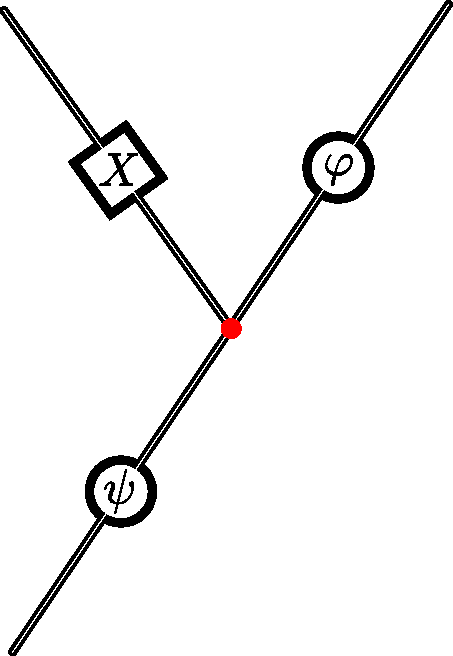
\includegraphics[scale = .50]{Vertex}
	\caption{The single vertex in our theory. It corresponds to the interaction $\langle \psi, [X,\varphi]\rangle$.}
\end{figure}

\begin{remark}[Going Under the Hood]
Now that we have an action of $\sL$ on $\E$, we would actually like to study the action of $\sL$ on $T^*[-1]\E$, which has a natural structure of a free theory. We want to be explicit about the pairing $\langle \cdot, \cdot \rangle$, as well as the operators $Q$ and $Q^{GF}$ in the cotangent theory to $\E$. The cotangent theory has space of fields
\begin{align*}
&\sV^{+,0} \overset{D^+}{\longrightarrow} \sV^{-,1}\\
&\oplus \quad\quad\quad \oplus\\
&\sV^{-,0}\overset{T}{\longrightarrow} \sV^{+,1},
\end{align*}
where we have used the metric $(\cdot,\cdot)$ to identify $V$ with $V^\vee$, and the Riemannian density to trivialize the density bundle. Once we specify the pairing $\langle, \rangle$ for our cotangent theory, $T$ will be determined by the requirement that $Q$ be skew-self-adjoint.

If $\psi \in \sV^!$, $\varphi \in \sV$, we let $\langle \psi, \varphi\rangle$ be the natural ``pair and integrate'' pairing. We note that this pairing comes with a minus sign when $\psi \in \sV^{!-}$ and $\varphi \in \sV^-$. The anti-symmetry of $\langle, \rangle$ requires that $\langle \varphi, \psi \rangle = -\langle \psi, \varphi \rangle$. To understand $D^{+!}$, we look at the requirement that the operator $Q = D^++D^{+!}$ be skew self-adjoint for $\langle \cdot, \cdot\rangle$. So, we let $\varphi \in \sV^+$, and $\psi \in \sV^{-!}$; then, we must have 
\[
\langle \psi , D^+ \phi \rangle = - \langle D^{+!}\psi, \phi\rangle,
\]
and in fact this serves as a definition of $D^{+!}$. Similarly, we would like to define $Q^{GF}= D^- +D^{-!}$; since $Q^{GF}$ must be self-adjoint for the invariant pairing, we have, assuming $\varphi \in \sV^-$ and $\psi \in \sV^{+!}$,
\[
\langle \psi , D^- \phi \rangle = - \langle D^{-!}\psi, \phi\rangle,
\]
where the minus sign appears because $\psi$ has cohomological degree 1. Again, this is sufficient to define $D^{-!}$. Finally, we want to define the action of $\sL$ on the fiber directions of $T^*[-1]\E$. Here, we require that the action preserve the pairing in the sense of Chapter 11 of \cite{ref: CG2}:
\[
\langle [X,\psi], \varphi\rangle = \langle [X,\varphi], \psi\rangle = -\langle \psi, [X,\varphi]\rangle.
\]
In other words, whenever we switch one of the operators $[X,\cdot]$, $Q$, $Q^{GF}$ from one side to the other, we always get a minus sign. This will be important to remember below.
\end{remark} 
\section{McKean-Singer}
Our main tool in proving formula \ref{eq: mcs} is the following theorem
\begin{theorem}[Gwilliam]
\label{th: og}
	\begin{enumerate}
		\item The obstruction to the $\L$-equivariant quantization of the cotangent theory to $\E$ is given by a well-defined cohomology class $\mathcal O\in H^\bullet(\widehat{Sym}(\L[1]^\vee))$.
		\item If the gauge-fixing is \textbf{positive} (in the sense of \cite[ref: othesis]), which is the case if in our key example $D$ is self-adjoint with respect to some Hermitian metric on $V$ and $M$ is compact, then for a closed form $\alpha\in \Omega^\bullet$, $\mathcal O(M)(\alpha)$ is given by the trace of the action of $H^\bullet(\L(M))$ on the determinant of $H^*(\E(M))$. Here we mean the graded determinant: if $V$ is a $Z$-graded vector space, 
		\[
		\det(V)=\bigotimes_{i} \left(\bigwedge^{\dim V_i}V_i\right)^{(-1)^i},
		\]
		with $W^{-1}$ defined as $W^\vee$.
	\end{enumerate}
\end{theorem}	
Now, we can describe how to compute the obstruction $\mathcal O(U)$. We make the following
\begin{definition}
	The \textbf{tree-level, scale t interaction} is the element $I_{tr}[t]$ of $\Obq[t]$ given by taking a sum over all connected tree-graphs with trivalent vertices as described above, with the propagator $Q^{GF}\int_0^t e^{-[Q,Q^{GF}]}$ inserted at each internal edge. In the language of \cite{ref: cost}, this is the $\epsilon \to 0$ limit of the mod $\hbar$ term of $W(P(\epsilon, L), I)$.
\end{definition}
Figure \ref{fig: trees} gives a diagrammatic depiction of $I_{tr}[t]$. As an example, the second diagram corresponds to the term
\[
(X,Y,\psi,\varphi)\mapsto \left\langle \psi, \left [ Y, Q^{GF}\int_0^t \exp{(-s[Q,Q^{GF}])}[X,\varphi]\right]\right\rangle,
\]
which we symmetrize over $X,Y$ to get the final contribution to $I_{tr}[t]$.
\begin{figure}[h]
\label{fig: trees}
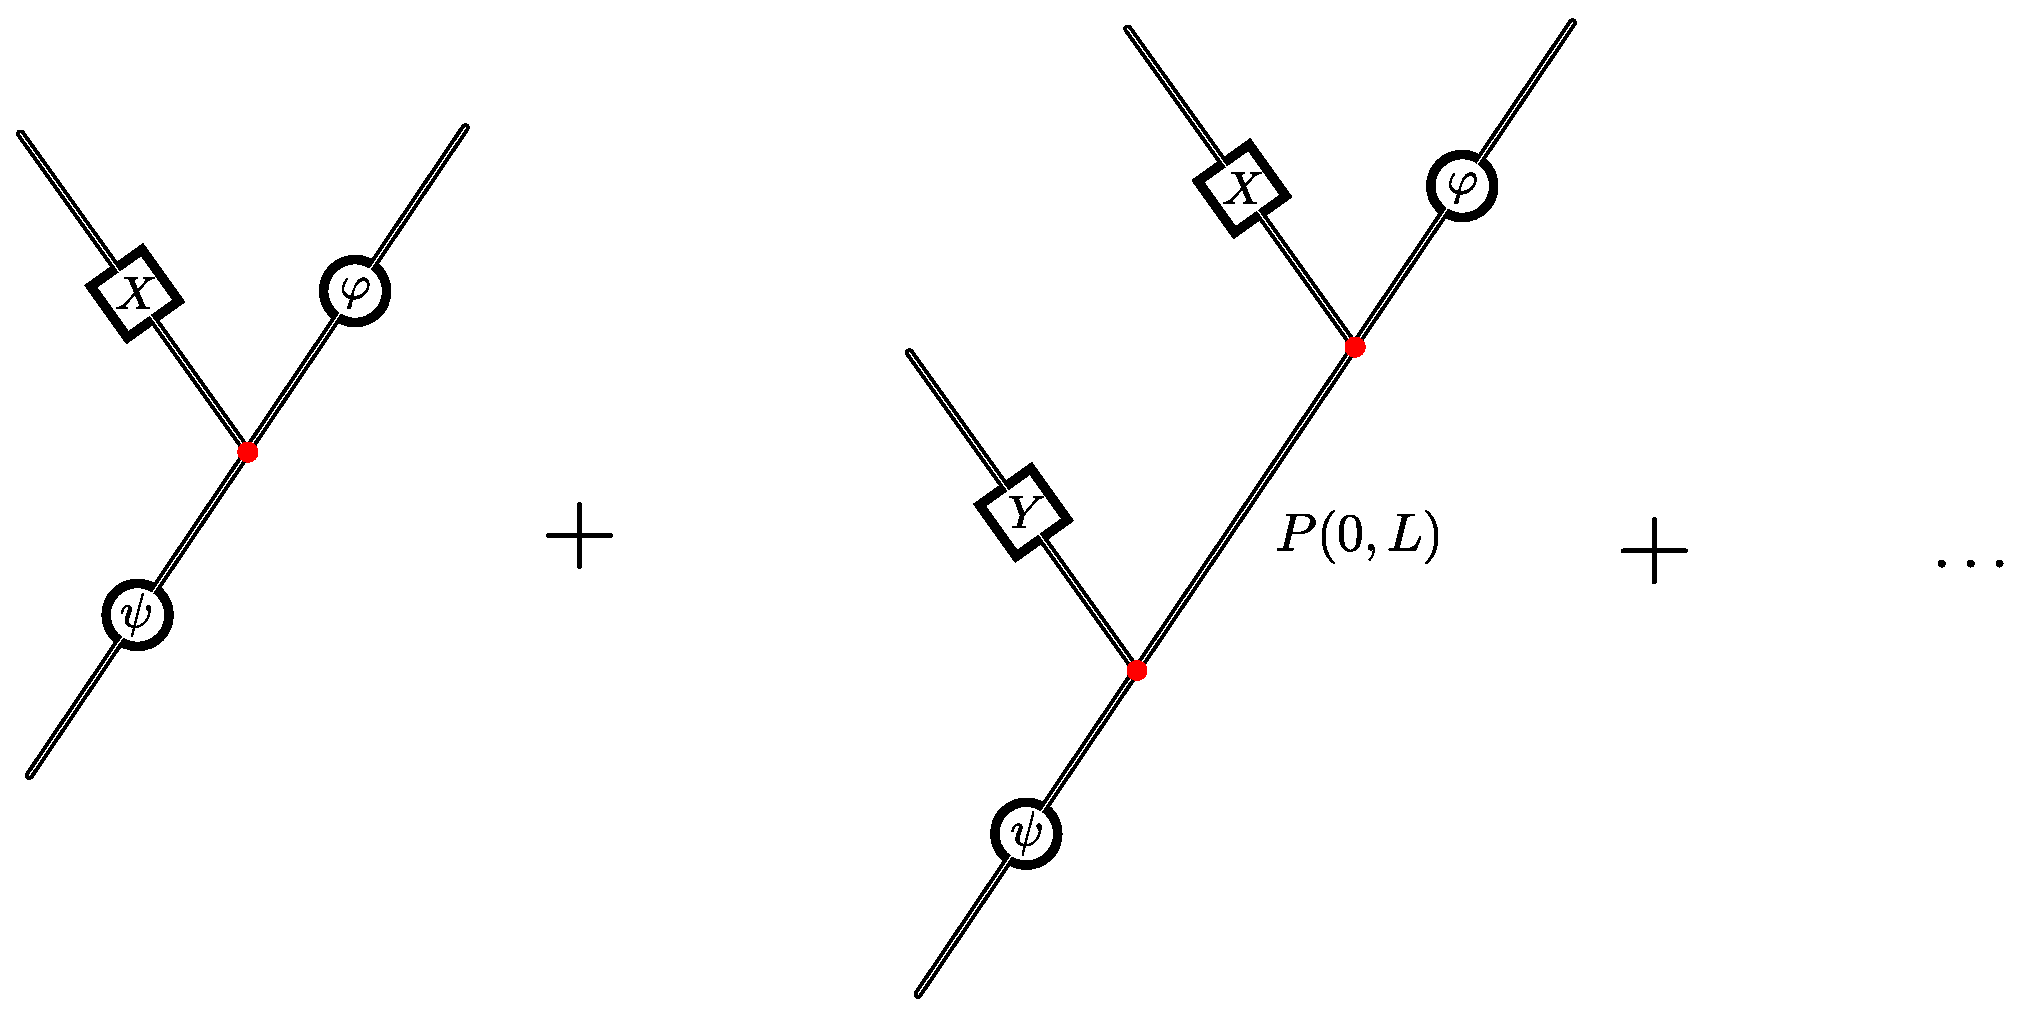
\includegraphics[scale = 0.4]{Trees}
\caption{The tree-level diagrams contributing to $I_{tr}[t]$.} 
\end{figure}
Notice that for simple combinatorial reasons, all of the trees contributing to $I_{tr}$ have only two external $T^{*}[-1]\E$ edges. Thus, $\Delta_t I_{tr}$ belongs to $\widehat{Sym}(\L[1]^\vee)$. 

Now that we have this definition in place, we can state, in addition to Theorem \ref{th: og}, the following
\begin{lemma}
	\label{lem: og}
	A representative of the obstruction class is given by $\Delta_tI_{tr}[t]$. The cohomology class of this obstruction is independent of $t$.
\end{lemma}

Notice that part (2) of Theorem \ref{th: og} and Lemma \ref{lem: og} give us two ways to evaluate the obstruction $\mathcal O$ on a closed form $\alpha$. Indeed, using these two ways, we will recover the McKean-Singer formula, to the proof of which we now turn.

\begin{proof}[Proof of Equation \ref{eq: mcs}]
We will use part (2) of Theorem \ref{th: og} and Lemma \ref{lem: og} to evaluate $\mathcal O(M)$ on a constant function $\lambda\in \R$. We should check that the gauge-fixing $D^-+D^{-!}$ is positive, but we defer this to the end of the proof.

Let us first work out what part (2) of Theorem \ref{th: og} tells us: in our case $H^\bullet(\E)$ has $\ker(D^+)$ in degree 0 and $\coker(D^+)$ in degree 1. Thus,

\begin{align*}
\det(H^\bullet(\E)\cong \bigwedge^{\dim\ker D^+}\ker D^+ \otimes \bigwedge^{\dim \coker D^+}(\coker D^+)^\vee.
\end{align*}

$\lambda$ acts on this one-dimensional space by multiplication by
\[
\lambda\left(\dim\ker(D^+)-\dim\coker(D^+)\right)=\lambda \ind (D).
\]
In other words, $\mathcal O(M)(\lambda) = \ind(D)$. This is the left-hand side of \ref{eq: mcs}.

On the other hand, let us study the Feynman diagrams appearing in $I_{tr}[t]$ with a $\lambda$ on each $\sL$ edge. A tree diagram with $n$ vertices gives, before symmetrization over $\sL$ inputs
\[
\lambda^n\left \langle \psi, \left(Q^{GF}\int_0^t e^{-s[Q,Q^{GF}]}ds\right)^{n-1} \varphi\right \rangle.
\]
However, since $I_{tr}[t]\in C^\bullet_{loc}(\sL)\otimes  C^\bullet_{loc}(\E[-1])$, it needs to be graded-symmetric over its $\sL$ inputs, and since $C^\bullet_{loc}(\sL)= \widehat Sym^\bullet (\sL[[1]^\vee)$, when we have a zero-form input $\lambda$ into $I_{tr}[t]$, all terms non-linear in $\lambda$ are anti-symmetrized away to zero. Thus, after applying $\Delta_t$ to $I_{tr}[t]$, we find that the only non-zero contribution to $\mathscr O(M)(\lambda)$ is represented by the ``tadpole'' diagram depicted in figure \ref{fig: tadpole}.
\begin{figure}[h]
\label{fig: tadpole}
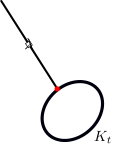
\includegraphics[scale = 0.5]{Tadpole}
\caption{The single diagram appearing in the Feynman diagram expansion for $\mathcal O(\lambda)$.}
\end{figure}

The tadpole diagram, evaluated on $\lambda$, gives 
\[
-\partial_{K_t}I_{tr}[t] = -\lambda\langle\cdot, \cdot \rangle (K_t\mid_\E),
\]
where we are restricting $K_t$ just to $\E$ from all of $T^*[-1]\E$ because the interaction takes only an $\E$ input into the first slot of $\langle, \rangle$, and a $\E^!$ input into the second. Thus, only the components of $K_t$ lying in $\E\otimes \E^!$ survive, and these are precisely the components we are considering when we take $K_t\mid_\E$. 

This is a good opportunity to review Costello's convention for $K_t$, which is subtly different from $k_t$ as defined and discussed above. By definition, $K_t$ is defined so that 
\[
-1\otimes \langle \cdot, \cdot \rangle(K_t\otimes s) = e^{-t[Q,Q^{GF}]}s,
\]
where $s\in T^*[-1]\E$. Let us denote by $k_t^+$ the heat kernel for the generalized Laplace operator $D^-D^+$, and similarly for the pairs $k_t^-$  and $D^+D^-$. Table \ref{tab: kernels} shows the bundles of which each is a section.
\begin{figure}[h]
\label{tab: kernels}
\begin{tabular}{c|c}
Heat Kernel & Section of \\
\hline\noalign{\smallskip}
$k_t^+$ & $V^+ \boxtimes V^{+\vee}$\\
$k_t^-$ & $V^- \boxtimes V^{-\vee}$
\end{tabular}
\caption{The two heat kernels and the bundles of which they are sections.}
\end{figure}
It therefore follows that 
\[
K_t\mid_\E = (-k_t^+-k_t^-)|dx| \in T^*[-1]\E \otimes T^*[-1]\E.
\] 
Finally, we wish to calculate
\[
\langle ,\rangle (K_t\mid_\E).
\]
In words, at each point $x\in M$, we take $K_t\mid_\E(x)$, which is an element of the fiber of $V\otimes V^!$ over $x$, we pair using the rules for $\langle , \rangle$, and we integrate the resulting density over $M$. But since we have $V$ on the left and $V^!$ on the right, we use the evaluation pairing with a minus sign, and we remember that the evaluation pairing comes with a minus sign for sections of $V^-\otimes V^{!-}$. Taking into account all of these factors, we have
\[
\langle ,\rangle (K_t\mid_\E)= \int_M \left(\Tr(k_t^+)-\Tr(k_t^-)\right)|dx| = \int_m \Str(k_t)|dx|,
\] 
which gives the right hand side of equation \ref{eq:mcs}.

The last thing we have to check is that $Q^{GF}$ is a \textit{positive} gauge fix. A positive gauge fix, by definition, needs to satisfy:

\begin{enumerate}
	\item The operator $H:= [Q,Q^{GF}]$ is symmetric for some Hermitian metric on the vector bundle $T^*[-1]E$.
	\item The eigenvalues of $H$ are non-negative.
	\item We have a direct sum decomposition 
	\[
	T^*[-1]\E = \ker H \oplus \text{im} Q \oplus \text{im} Q^{GF}.
	\]
	This decomposition is as topological vector spaces.
\end{enumerate}
Item 1 is satisfied by assumption, item 2 is satisfied because $H$ is the square of a self-adjoint operator, and item 3 follows from the statement and proof of proposition 3.48 in \cite{ref: bgv}.
\end{proof}
\section{More Feynman Diagrams}
We have our desired result; however, we have only evaluated the obstruction $\mathcal O$ on a constant function $\lambda$. What happens when we evaluate this obstruction on an element $\lambda+\alpha$, where $\alpha$ is a closed 1-form? Well, since $\alpha$ acts off-diagonally on $\E$, part (2) of \ref{th: og} still gives us $2\lambda\ind(D)$. However, the Feynman diagrammatics look \textit{a priori} very different. There is now no reason to rule out more complicated tree diagrams from appearing. However, we do still have the following 

\begin{proposition}
For $\lambda\in \R$, $\alpha \in \Omega^1(M)$, the Feynman diagram expansion of $\Delta_tI_{tr}[t](\lambda +\alpha)$ gives $\int_M \Str k_t |dx|$.
\end{proposition}

\begin{proof}
It is easy to see for degree reasons that the only tree diagrams giving a non-zero contribution to $I_{tr}[t]$ are those with $\lambda$ on one of the external $\sL$ edges (which we will now call ``legs'') and $\alpha$ on all the rest. Now, the diagram with one leg gives the term $\lambda \int_M \Str k_t(x,x) |dx|$, as we saw above. So, we need to show that all the other diagrams give zero. Let's focus first on the two-leg diagrams; the higher-leg diagrams will vanish for very similar reasons. One of the two two-leg tree diagrams is depicted in Figure \ref{fig: twoleg}; the other is given by exchanging $\lambda$ and $\alpha$.

\begin{figure}[h]
\label{fig: twoleg}
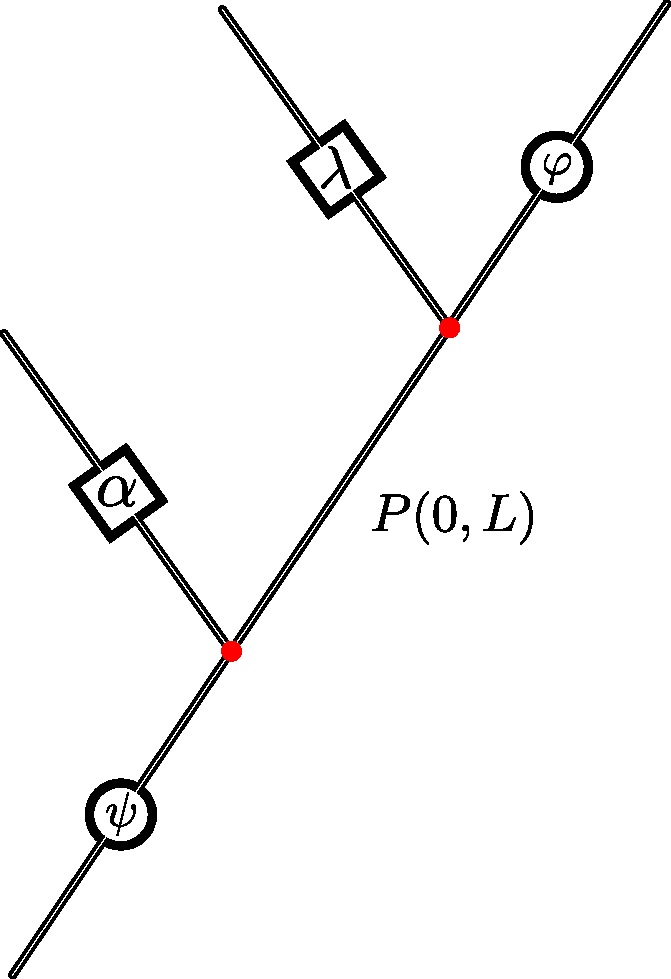
\includegraphics[scale = 0.50]{TwoLegs}
\caption{One of the two two-leg, tree-level diagrams contributing to $I_{tr}[t]$. The other one is given by exchanging $\lambda$ and $\alpha$.}
\end{figure}
The contribution from these two diagrams is given by the term
\[
\lambda\left(\langle \psi,[\alpha, P\varphi]\rangle+\langle \psi,P[\alpha, \varphi]\rangle  \right), 
\]
where $\psi \in \E$ and $\varphi \in \E^!$. Recall that whenever we move $[\alpha, \cdot]$, $Q$, and $Q^{GF}$ from one side of the pairing to the other, we pick up a minus sign. Since $P= Q^{GF}\int_0^t e^{-s[Q,Q^{GF}]}ds$, and since $Q^{GF}$ and $[Q,Q^{GF}]$ commute, we also pick up a minus sign in moving $P$ from one side of the pairing to the other. Thus, the two-leg tree diagrams contribute

\[
\lambda\left(\langle P[\alpha,\psi],\varphi\rangle+\langle \psi,P[\alpha, \varphi]\rangle  \right)=\lambda\left(-\langle\varphi, P[\alpha,\psi]\rangle+\langle \psi,P[\alpha, \varphi]\rangle  \right). 
\]
In other words, this contribution is anti-symmetric under the transposition of its two inputs. We need to show that when evaluated on $K_t$, this contribution gives 0.

It is not hard to extend this argument to the higher-leg terms; there, the $n$-leg diagrams give the following contribution
\[
\lambda\left(\langle \psi, ([\alpha,\cdot] P)^{n-1}\varphi \rangle +\langle \psi, ([\alpha,\cdot] P)(P[\alpha,\cdot])^{n-2}\varphi \rangle+\cdots+\langle \psi, (P[\alpha,\cdot])^{n-1}\varphi \rangle\right).
\]
Since all but the first and last terms involve $P^2=0$, only the first and last terms need to be shown to be zero. But this argument is entirely analogous to the one for two-leg diagrams.
\end{proof}
\section{Equivariant McKean-Singer}
We would like to generalize the set-up of our problem in the following way: suppose we have a Lie algebra $\fg$ acting on $V$ by (self-adjoint) even operators and that this action commutes both with the $\cinfty$ action and with $D$. In other words, we have a Lie algebra map
\[
\rho: \fg \to \Gamma(\End_{(s.a.)}^0(V))
\]
such that $\rho(\gamma)(Ds)=D\rho(\gamma)(s)$ for all $s\in \sV$, $f\in \cinfty(M)$, and $\gamma\in \fg$. 
\begin{remark}
	Since the equation of motion of the free theory we are considering is essentially $D\varphi = 0$, we are to think of $\fg$ as a Lie algebra of symmetries of our theory. After all, if $D\varphi =0$, then $D((1+\gamma)\varphi)=D\varphi +D\gamma \varphi = 0+\gamma D\varphi = 0$, so that $\gamma$ infinitesimally preserves the equation of motion. In physics lingo, the obstruction $\mathcal O$ is the \textit{anomaly}, the measure of the violation of the symmetry at the quantum level. 
\end{remark}
We will usually just denote the action of an element $\gamma\in \fg$ on a section $s\in \sV$ by $\gamma.s$. Since $\gamma$ commutes with $D$, it preserves $\ker D^+$ and $\coker D^+$, so we are free to make the following
\begin{definition}
	Let $\fg$ act on $V$ as above. Then, the \textbf{equivariant index} of $D$ is the following function on $\fg$:
	\[
	\ind(\gamma, D)= \Tr(\gamma\mid_{\ker D^+})-\Tr(\gamma\mid_{\coker D^+}).
	\]
\end{definition}
With this definition in hand, we can now state the \textbf{equivariant McKean-Singer theorem}:
\begin{theorem}
\begin{equation}
	\label{eq: eqmcs}
	\ind(\gamma, D) = \int_M \Str(\gamma k_t(x,x))|dx|.
\end{equation}
\end{theorem} 
Note that in the special case where $\fg = \R$ and the action is given by scalar multiplication, this theorem just reproduces the regular McKean-Singer formula.

We will see that our proof of the regular McKean-Singer formula carries over \textit{mutatis mutandis} to the equivariant case, once we carry out the due diligence of constructing a local action of $\fg\otimes \Omega^\bullet$ on $\E$. Since this is elliptic $L_\infty$ algebra with which we are now pre-occupied, we will use $\sL$ to denote its sheaf of sections. This is the work to which we now turn:
\begin{proposition}
There is a unique central extension of elliptic dglas 
\[
0\to \E \to \sL \oplus \E \to \sL \to 0
\]
satisfying 
\begin{enumerate}
\item $[x,y]_{\sL\oplus \E}=[x,y]$ if $x$ and $y$ are both in $\sL$ or both in $\E$. We are viewing $\E$ as an abelian elliptic dgla.
\item For $\gamma\in \fg$ and $\varphi\in \E$, $[\gamma\otimes 1, \varphi] = \gamma.\varphi$, so that the action of $\sL$ on $\E$ coincides with the action of $\fg$ for elements of $\fg\otimes 1$.
\item The map
\[
[,]: \sL \otimes \E \to \E
\]
is $\cinfty$-bilinear.
\end{enumerate}
\end{proposition}
\begin{proof}
For degree reasons (as before), we need only to specify a degree zero action of functions and a degree 1 action of one-forms satisfying
\begin{align*}
D^+([X,\varphi]) &= [dX,\varphi] +(-1)^{|X|}[X,D^+\varphi]\\
[X,[Y,\varphi]] &= [[X,Y],\varphi] +(-1)^{|X||Y|}[Y,[X,\varphi]].
\end{align*}
for all $X,Y\in \sL$ and $\varphi \in \E$. Items 2) and 3) in the statement of the proposition tell us that for elements of $\sL$ of the form $\gamma \otimes f$ with $f\in \cinfty$, we must have
\[
[\gamma\otimes f, \varphi] = f\gamma.\varphi.
\]
On the other hand, for elements of $\sL$ of the form $\gamma\otimes df$, the derivation property requires that
\begin{equation}
\label{eq: 0form}
[\gamma\otimes df,\varphi]= D^+(f\gamma.\varphi)-f\gamma.(D^+\varphi)=\gamma.([D^+,f]\varphi),
\end{equation}
where we have used the fact that $\gamma$ commutes with $\cinfty$ functions and $D^+$. Just as above, this fixes the action of one-forms on $\E$. More precisely, if we denote by $c(\alpha)$ the action of the one-form $\alpha$ on $\E$ defined in Proposition \ref{prop: action}, then the action of an element $\gamma\otimes \alpha$ of $\sL$ on an element $\varphi$ of $\E$ is given by
\begin{equation}
\label{eq: 1form}
[\gamma\otimes \alpha, \varphi] = \gamma.(c(\alpha)\varphi).
\end{equation}

Equations \ref{eq: 0form} and \ref{eq: 1form} define the bracket $\sL\otimes \E \to \E$, and we have just argued for its uniqueness. It remains to verify the Jacobi identity, since we have already extracted all of the non-trivial information from the derivation property. For degree reasons, the Jacobi identity is trivially satisfied as long as both $X$ and $Y$ are of non-zero degree. So it suffices to check the Jacobi identity for $X = \gamma_1 \otimes f$ and $Y= \gamma_2\otimes g$ or $\gamma_2 \otimes \alpha$ where $f,g\in \cinfty$ and $\alpha \in \Omega^1$. In the first case, we have
\begin{align*}
[\gamma_1\otimes f,[\gamma_2\otimes g,\varphi]]&=fg\gamma_1.\gamma_2.\varphi\\
[[\gamma_1\otimes f, \gamma_2 \otimes g],\varphi]+[\gamma_2\otimes g, [\gamma_1\otimes f, \varphi]]&=fg[\gamma_1,\gamma_2].\varphi + fg\gamma_2.\gamma_1.\varphi,
\end{align*}
and we see that the Jacobi identity is satisfied because $\fg\to \Gamma(\End^0(V))$ is a Lie algebra homomorphism. In the second case, we have
\begin{align*}
[\gamma_1\otimes f,[\gamma_2\otimes \alpha,\varphi]]&=fg\gamma_1.\gamma_2.(c(\alpha)\varphi)\\
[[\gamma_1\otimes f, \gamma_2 \otimes \alpha],\varphi]+[\gamma_2\otimes \alpha, [\gamma_1\otimes f, \varphi]]&=f[\gamma_1,\gamma_2].(c(\alpha)\varphi) + f\gamma_2.(c(\alpha)\gamma_1.\varphi).
\end{align*}
Because $c(\alpha)$ is defined using only the actions of $D^+$ and $\cinfty$ on $\E$, $c(\alpha)$ commutes with $\gamma_1$, and so the last term in the above equation is $\gamma_2.\gamma_1(c(\alpha)\varphi)$. Just as for the first case, then, the Jacobi identity is satisfied.
\end{proof}

Now, we proceed just as above to prove Equation \ref{eq: eqmcs}:
\begin{proof}[Proof of Equation \ref{eq: eqmcs}]
	We evaluate the obstruction class on an element $\gamma\otimes 1$ using Lemma \ref{lem: og} and Theorem \ref{th: og}.	Just as for the non-equivariant formula, for symmetry reasons, only one diagram contributes to the Feynman diagrammatics, and that diagram gives a contribution
\[
\int_M \Str(\gamma k_t(x,x))|dx|.
\]

On the other hand, $\gamma\otimes 1$ acts on $\det \ker (D^+)$ by $\Tr(\gamma\mid_{\ker D^+})$ and similarly for $\det (\coker(D^+)^\vee)$, so that the application of Theorem \ref{th: og} gives us 
\[
\mathcal O (M)(\gamma\otimes 1) = \ind(\gamma, D).
\] 
\end{proof}

\section{Maturer Statements}
There is a much cleaner theoretical language in which to understand these results, based on the following nice characterization of the obstruction complex $C^\bullet_{loc}(\Omega^\bullet_{dR}(M))$. We will assume in this section that $M$ is orientable, so that there is no difference between densities and volume forms. 
\begin{lemma}[Non-Equivariant Obstruction Complex]
	\label{lem: qism}
	The map \[\Omega^\bullet(M) [n-1]\to J(\Omega^\bullet_{dR}(M))^\vee[-1] \hookrightarrow C^\bullet_{loc}(\Omega^\bullet_{dR}(M))\] given by
	\[
		\alpha \mapsto \left( \beta \mapsto \int_M \alpha \wedge \beta\right)
	\]
	is a quasi-isomorphism.
\end{lemma} 
\begin{proof}
We first recall that one definition of $C^\bullet_{loc}$ is
\[
C^\bullet_{loc}(\Omega^\bullet_{dR}(M)) = \text{Dens}_M\otimes_{D_M} C^\bullet_{red}(J(\Omega^\bullet_{dR})(M)),
\]	
where $J(\Omega^\bullet_{dR}(M))$ is the space of global sections of the (infinite) jet bundle of $\Omega^\bullet_{dR}$ and the subscript \textit{red} means that we quotient out by the $\Sym^0$ piece of $C^\bullet$. In our case, since the $L_\infty$-algebra we're considering is abelian, $C^\bullet_{red}(J(\Omega^\bullet_{dR})$ is just $\Sym^{>0}(J(\Omega^\bullet_{dR})^\vee[-1])$ with the differential induced by the de Rham differential. 

We will replace both terms in the (derived) tensor product defining the obstruction complex with quasi-isomorphic complexes. Let's start with the map of $D_X$ modules
\[
C^\infty_X \hookrightarrow J(\Omega^\bullet_{dR})
\]
The Poincar\'{e} lemma can be used to show that this is a quasi-isomorphism of $D_X$ modules. Namely, letting $(\alpha, U)$ be a representative of the germ of a closed cohomological degree $d$ section of the bundle $J(\Omega^\bullet_{dR}$ at a point $p$, and assuming that $U$ is homeomorphic to $\R^n$, the Poincar\'{e} Lemma tells us that $\alpha$ is exact on $U$ unless $d=0$, in which case $\alpha$ is cohomologous to the jet of a constant function. Thus, the above map is a quasiisomorphism of $D_X$ modules, and it follows that we have a quasi-isomorphism 
\end{proof}

The main result of this section is
\begin{theorem}
Under the quasi-isomorphism of \ref{lem: qism}, the obstruction $\mathcal O(M)$ corresponds to $ \Str k_t(x,x)|dx|$.	
\end{theorem}
\begin{proof}
	content...
\end{proof}
\begin{thebibliography}{99}
\bibitem[G12]{ref: othesis}
Gwilliam, Owen. Factorization Algebras and Free Field Theories. PhD Thesis. 2012.
\bibitem[CG16]{ref: CG2}
Costello, Kevin, and Gwilliam, Owen. Factorization Algebras and Quantum Field Theory, Volume 2. \url{http://people.mpim-bonn.mpg.de/gwilliam/vol2may8.pdf}, 2016.
\bibitem[Cos11]{ref: cost}
Costello, Kevin. Renormalization and Effective Field Theory. American Mathematical Society, 2011.
\bibitem[BGV04]{ref: bgv}
Berline, Vergne, Getzler.
\end{thebibliography}
\end{document}